\documentclass[11pt]{article}

\usepackage[a4paper,margin=2.5cm]{geometry}
\usepackage{amsmath}
\usepackage{graphicx}
\usepackage{xcolor}
\usepackage[font=small,labelfont=bf]{caption}
\usepackage{float}
\usepackage{enumitem}
\usepackage{microtype}
\usepackage[hidelinks]{hyperref}

\definecolor{lensorange}{HTML}{D98A00}
\definecolor{lensslate}{HTML}{3A3A42}
\definecolor{lensblue}{HTML}{4F7BF6}
\definecolor{lenspaper}{HTML}{F9F9FA}
\hypersetup{colorlinks=true,linkcolor=lensslate,urlcolor=lensblue}
\setlength{\parindent}{0pt}\setlength{\parskip}{0.6em}

\newcommand{\takeaway}[1]{\begin{center}
  \fcolorbox{lensslate}{lenspaper}{\parbox{0.95\linewidth}{\small\textbf{\color{lensorange}Takeaway.}\ #1}}\end{center}}

\title{\vspace{-1.4cm}
  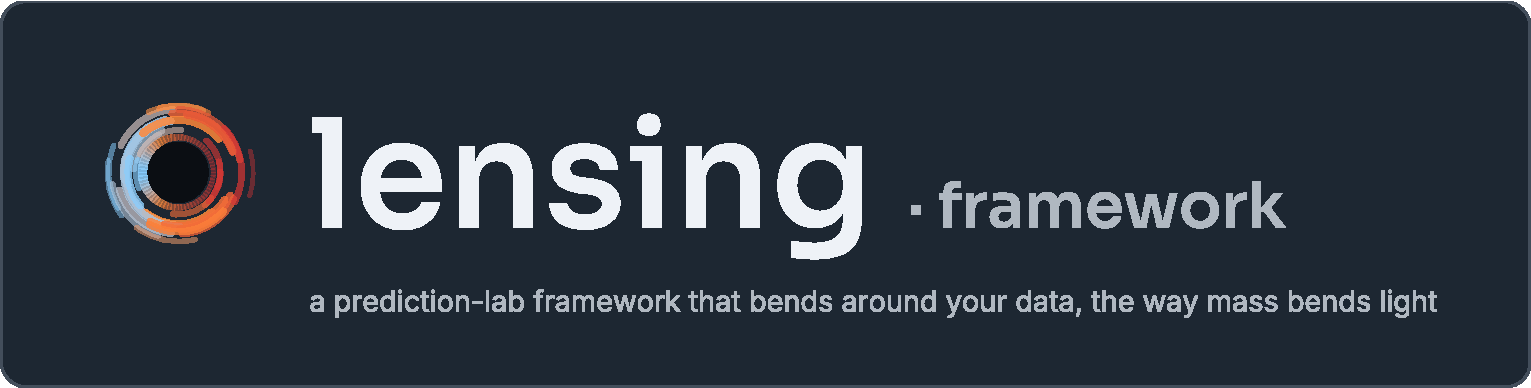
\includegraphics[height=1.25cm]{assets/lensing-logo.pdf}\\[0.7em]
  \textbf{Pathfinder, in Plain Terms}\\[0.2em]
  {\large What the Models Do, Why, and What We Learned}}
\author{\textsc{lensing}\,\,$\cdot$\,\,spotify-pathfinder \quad\small(product \& concept overview)}
\date{June 2026}

\begin{document}
\maketitle

\begin{abstract}\noindent
Pathfinder turns two songs into a \emph{journey}: pick a start track and an end track, and it builds a
playlist that glides from one to the other, shown as a path through a 3D ``map'' of musical taste.
This overview explains, without heavy math or code, what the pieces are, the decisions behind them,
and the most useful things we learned --- including a couple of findings that are good reminders for
any ML product. A companion engineering guide and a full technical paper cover the details.
\end{abstract}

%====================================================================
\section{What it does}
You give it two Spotify tracks. It finds a sequence of songs --- a ``musical procession'' --- that
moves smoothly from the first to the second, and draws that path threading through a cloud of nearby
tracks in 3D. You can play 30-second previews back-to-back, or save the route as a real Spotify
playlist. Everything runs on a single, cheap, serverless function; there is no always-on server and no
database humming in the background.

%====================================================================
\section{How it works, conceptually}
Three ideas do the work.

\textbf{1. A map of taste.} Every song in the library (about 23{,}500 of them) is placed as a point on
a map, positioned so that songs that \emph{feel} similar sit close together. The map has many
invisible dimensions, but the picture you see is a faithful 3D shadow of it. ``Distance'' on this map
is the app's notion of how different two songs are.

\textbf{2. A smart route, not a straight line.} Getting from song A to song B is a navigation problem.
The app prefers steps that are short on the map, land on songs people tend to stick with, follow
pairings real listeners actually make, and suit the moment (morning vs.\ night, shuffle vs.\ a
deliberate sit-down listen) --- while avoiding repeats and too much of one artist. It balances these
preferences to pick a pleasing path.

\textbf{3. It all runs at the edge.} Rather than keep heavy machine-learning models running, we do all
the learning \emph{ahead of time} and bake the \emph{results} into a small data file that ships with
the app. At request time the app just reads that file and does fast arithmetic.

\takeaway{The serverless function gets only about 10 milliseconds of compute per request. That budget
is why we precompute everything: the models produce data offline; the live app only does lightweight
navigation over that data. It is cheaper and simpler to run, at the cost of a periodic rebuild when the
music library changes.}

%====================================================================
\section{The ``fit'' score: will you come back to a song?}
One ingredient deserves a closer look because it drives which songs the route favors. For every track
we predict a \textbf{fit} score: roughly, \emph{how likely you are to play this song again} (we
defined ``a keeper'' as a track played at least twice). A standard, well-understood model
(gradient-boosted trees) makes this prediction.

How good is it? It reaches an \textbf{AUC of about 0.74}. AUC runs from 0.5 (a coin flip) to 1.0
(perfect); 0.74 means that, given one keeper and one non-keeper, the model ranks the keeper higher
about three times out of four --- a solid, useful signal from song attributes alone, not magic.

%====================================================================
\section{Two findings worth remembering}

\textbf{Finding 1: who made it beats what it sounds like.} The intuitive approach is to describe each
song with rich ``fingerprints'' --- audio features, text descriptions, learned embeddings. We tried
all of those. They \emph{did not help}; some made the prediction worse. What worked was simple
\emph{identity}: which artist, which genre. Plain identity, fed to decision trees, beat every fancier
model we tested (Figure~\ref{fig:bakeoff}).

\begin{figure}[H]\centering
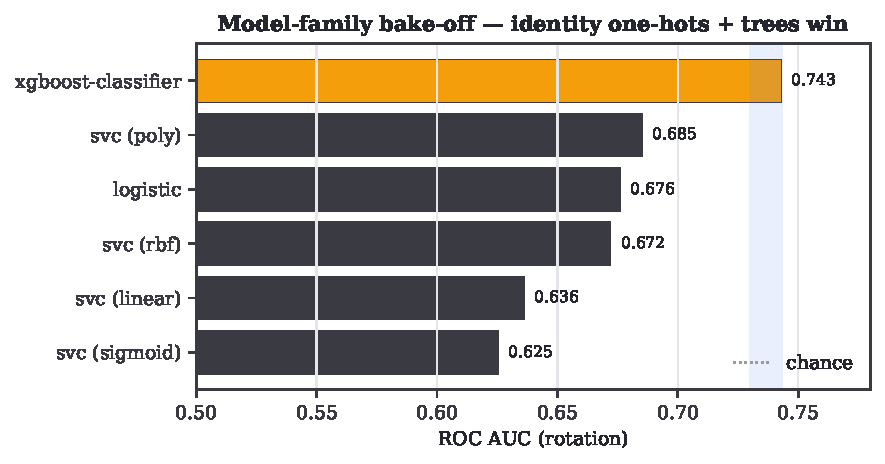
\includegraphics[width=0.74\linewidth]{figures/fig_bakeoff.pdf}
\caption{Each bar is a different modeling approach; higher is better. The simple ``artist/genre
identity + trees'' model (orange) wins clearly. The fancier distance- and margin-based models all
trail it.}
\label{fig:bakeoff}
\end{figure}

\textbf{Finding 2: tuning the model barely moved the needle.} It is tempting to spend time tuning a
model's knobs. We ran that tuning sweep on the real data; the best setting beat our default by an
amount \emph{smaller than the natural run-to-run noise} (Figure~\ref{fig:xgb}). In other words, the
default was already good enough, and effort is better spent on the data than on knob-twiddling.

\begin{figure}[H]\centering
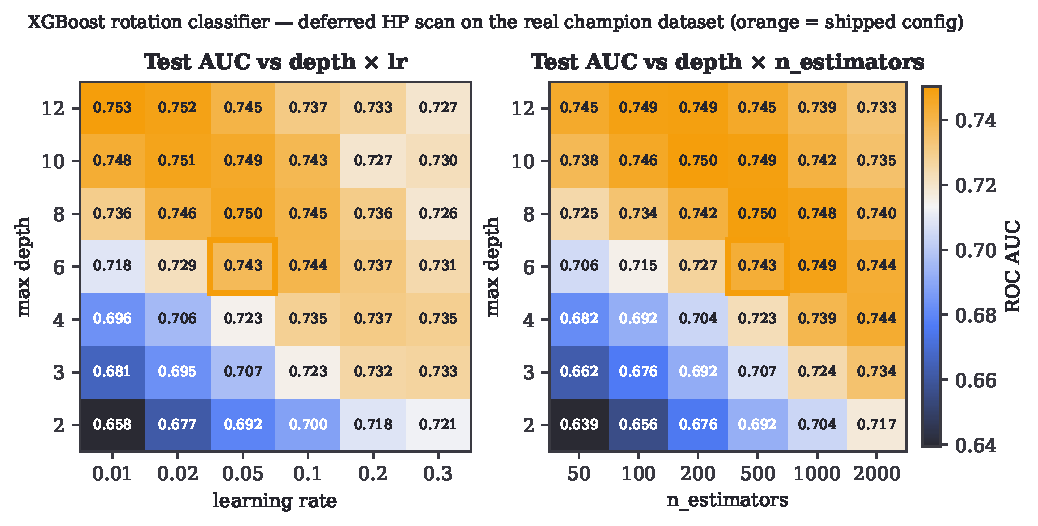
\includegraphics[width=\linewidth]{figures/fig_xgb_sweep.pdf}
\caption{Each square is one tuning setting; warmer is better. The shipped setting is outlined. Plenty
of squares look slightly warmer, but the differences are within the measurement noise --- tuning was
not the lever that mattered.}
\label{fig:xgb}
\end{figure}

\takeaway{Across both findings: in this problem, \emph{features and data choices} mattered far more
than model sophistication or tuning. A useful prior for the next ML feature: get the inputs right
before reaching for a bigger model.}

%====================================================================
\section{Listening has a rhythm}
The app also learns \emph{when} you reach for different music, and uses it. We measure a ``lift'': how
much more (or less) a kind of music shows up in a given context than usual --- a lift of 2 means
``twice as common here'', 1 means ``no difference'', below 1 means ``less common''.

The patterns are real and intuitive (Figure~\ref{fig:lifts}, left): some genres are morning music,
others are night music; some are played in deliberate, in-order sessions while others surface on
shuffle. Interestingly, when we ran the \emph{same} analysis on a song's release era (Figure~\ref{fig:lifts},
right), the effect almost vanished: \emph{what kind} of music you reach for changes a lot by time of
day, but \emph{when it was made} hardly does. Not every attribute carries a useful signal --- a handy
thing to check before building a feature around one.

\begin{figure}[H]\centering
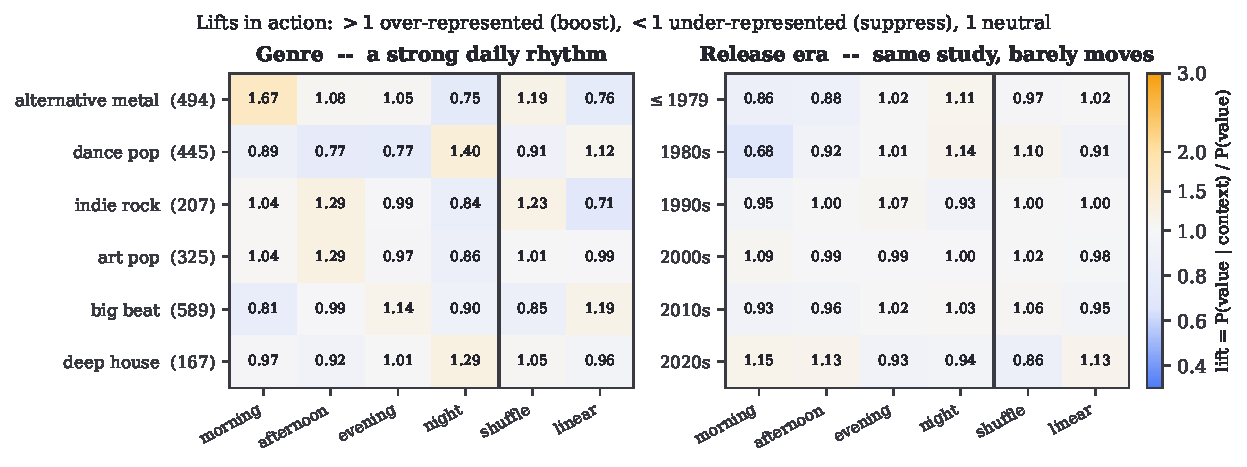
\includegraphics[width=\linewidth]{figures/fig_lifts.pdf}
\caption{How over- or under-represented something is in a context (orange = more than usual, blue =
less, near-white = no effect). Left: musical genre swings strongly with time of day and shuffle.
Right: the song's release era, analyzed the same way, barely budges.}
\label{fig:lifts}
\end{figure}

%====================================================================
\section{Songs the app has never seen}
What if you pick a song that is not on the map? The app handles this ``cold start'' by looking the
track up on Spotify, building a quick description of it, and estimating where it \emph{would} sit on
the map, then snapping it to the nearest known song and routing from there. It is an approximation, so
the app is honest about it: it tells you it snapped your pick to a nearby track.

%====================================================================
\section{What we learned, and honest limits}
\begin{itemize}[leftmargin=1.4em,itemsep=3pt]
\item \textbf{Right inputs beat bigger models.} Identity features won; fancy embeddings and extra
tuning did not move the result beyond noise.
\item \textbf{Precomputing buys simplicity.} Doing the heavy work offline lets the whole product run
on one tiny serverless function --- the trade is a rebuild whenever the library changes.
\item \textbf{Context is about genre, not era.} Time of day and shuffle strongly shape \emph{what kind}
of music fits; release era barely matters.
\item \textbf{Known limits.} The ``fit'' model is good, not perfect (${\sim}0.74$ AUC); the taste signal
it can't explain is personal and behavioral. The patterns above come from one listener's history, so
they describe \emph{this} library, not music in general. And on the free serverless tier, very
far-apart song pairs can exceed the compute budget and return ``no route found'' rather than a bad
one.
\end{itemize}

For the engineering walkthrough (how the runtime and data fit together) see \emph{Pathfinder, for
Engineers}; for the full methodology and equations see \emph{The Models of Pathfinder}.

\end{document}
